\subsection[An Algorithm with Performance Guarantees]{A Practical Algorithm with Performance Guarantees for the Art Gallery Problem \cite{DBLP:journals/corr/abs-2007-06920}}
Hengeveld and Miltzow \cite{DBLP:journals/corr/abs-2007-06920} introduce the idea of vision-stability, and describe an iterative algorithm that guarantees to find the optimal guard set for every vision-stable polygon in order to address the Art Gallery Problem \cite{o1987art}. Additionally, it proves that the set of vision-stable polygons admits an FPT algorithm when parametrised by the number of vertices visible from a chord of the polygon, and gives a one-shot algorithm for that matter.

Hengeveld and Miltzow \cite{DBLP:journals/corr/abs-2007-06920} start by introducing the notion of vision-stability (see Figure \ref{fig:vis}). The figure was taken from \cite{DBLP:journals/corr/abs-2007-06920} and annotated to facilitate the understanding of this summary. The authors define guards as ``enhanced'' if they can ``see around the corner'' by an angle of $\delta$ ($vis_\delta(p)$), or ``diminished'' if their vision is ``blocked'' by reflex vertices by an angle of $\delta$ ($vis_{-\delta}(p)$). As such, the size of the minimum $\delta$-guarding set is defined as $opt(P, \delta)$. A polygon $\mathcal P$ has vision-stability $\delta$ if the optimal number of enhanced guards is the same as the optimal number of diminished guards for that matter ($opt(P, -\delta) = opt(P, \delta)$). 

\begin{figure}[h!]
    \centering
    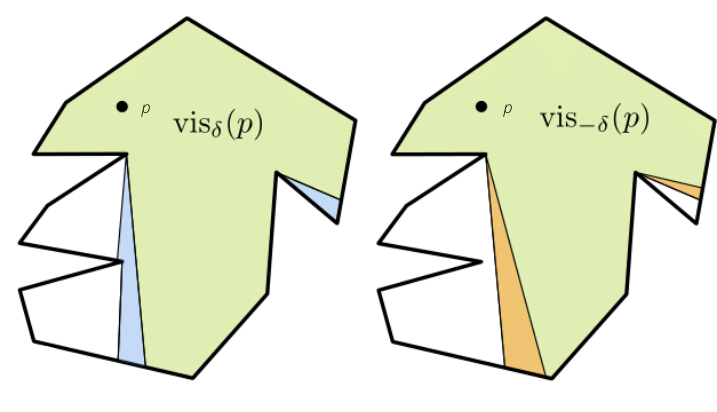
\includegraphics[width=0.5\textwidth]{literature/vis_delta.png}
    \caption{Enhanced ($vis_\delta(p)$) and Diminished ($vis_{-\delta}(p)$) Visibility Regions of $p$ \cite{DBLP:journals/corr/abs-2007-06920}.}
    \label{fig:vis}
\end{figure}

The core idea of Hengeveld and Miltzow's approach is to discretise the problem in order to improve the computation time. In this way, only a subset of potential guards and points to be guarded from $\mathcal P$ would be considered. In order to do so, they introduce the notions of a candidate guard set $C$ and a witness set $W$. The role of the candidate guard set $C$ is to discretise the guard searching space. As such, we can find an upper bound $opt[C]$ on the final guard set. Thus $C$ is ``pretty close'' on the actual optimum guard set $opt$. The candidate guard set $C$ is then initialised with a subset of all the potential guards. The guards that are included should have their visibility regions overlap as little as possible. Similarly, the witness set $W$ discretises the space of the guards' visibility regions. At initialisation time, $W$ contains a subset of all vertices and faces of $\mathcal P$. It is important to also include faces in $W$. In this way, we account for the fact that if a point $p$ is included in a face $f$, then $f$ sees at least as much as $p$. So, we can determine an approximation of how much more $f$ sees when compared to $g$. Thus, by adding the face as a witness, we are creating a discretisation of the space containing a superset of possible guard positions.

Firstly, rays are shot from every reflex vertex such that the angle between any two rays is at most $\delta$, as observed in Figure \ref{fig:rays}, as taken from \cite{DBLP:journals/corr/abs-2007-06920}. All the intersection points of the rays within $\mathcal P$ define the candidate guard set $C$, together with the faces they are part of. A witness guard set $W$ is then defined by picking an arbitrary interior point of every face of $\mathcal P$, together with all faces of $\mathcal P$. In this way, the problem can be discretised in a way in which the solution to the discretised problem are also solutions to the continuous problem.

\begin{figure}[h!]
    \centering
    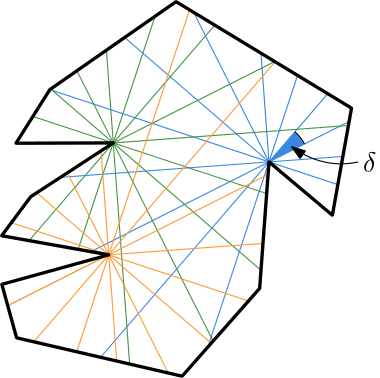
\includegraphics[width=0.3\textwidth]{literature/Shooting-1.png}
    \caption{Shooting rays from all reflex Vertices with angles between them at most $\delta$ \cite{DBLP:journals/corr/abs-2007-06920}.}
    \label{fig:rays}
\end{figure}

\newpage
\subsubsection{One-Shot Vision-Stable Algorithm}
At first, an Integer Program (IP) is built and named the One-Shot Vision-Stable Algorithm. It computes the minimum number of point guards in polynomial time in a vision-stable polygon $\mathcal P$ with  vision-stability $\delta$ and $r$ reflex vertices. The guards are encoded by binary integers, and linear equations and inequalities are used to encode visibility. Assuming that $\delta$ is part of the input, the algorithm returns the optimal solution only if the vision-stability of $\mathcal P$ is larger or equal to $\delta$. The one-shot vision-stable algorithm is reliable, as it also verifies that its result is an optimal solution. 

Let $f_1$ be the optimisation fuction of the IP. The function $f_1$ uses variables $[[c]]$ for every candidate $c \in C$, and $[[w]]$ for every witness $w \in W$. Its role is to count the number of guards that are used with the purpose of minimising this number. Additionally, it makes use of parameter factor $1 + \varepsilon$  to ensure that vertex candidates are preferred over face candidates. By choosing $\frac 1 \varepsilon = |C| + |W| + 1$, we ensure that $\varepsilon$ is sufficiently small. As such, the optimisation function $f_1$ of the IP is 
$$f_1 = \sum_{c \in \text{vertex}(C)} [[c]] + (1 + \varepsilon)\sum_{c \in \text{face}(C)} [[c]] + \varepsilon \sum_{w \in \text{face}(W)} [[w]].$$
For every witness $w$, its visible set of candidates are denoted as $vis(w)$, where $face$ and $vertex$ refer to whether the candidate is a face or a vertex, respectively.

Additionally, let $\text{vis}(w)$ be the set of candidates that see witness $w \in W$ completely. For every vertex-witness $w \in \text{vertex}(W)$, we formulate a constraint such that all $w \in \text{vertex}(W)$ is seen: $$\sum_{[[c]] \in vis(w)} c \geq 1, \forall w \in \text{vertex}(W).$$ We similarly formulate a constraint for every face-witness $w \in \text{face}(W)$. However, we add $[[w]]$ as a variable to relax it, so that the focus is placed on first seeing all vertex-witnesses $$[[w]] + \sum_{[[c]] \in vis(w)} c \geq 1, \forall w \in \text{face}(W).$$

% for each vertex and face witness $w$ to be respectively seen by all candidates from $vis(w)$ is added. 
% % \begin{equation}
% 	\begin{align*}
% 		\sum_{c \in Vis(w)} c &\geq 1, \forall w \in \text{vertex}(W) \\
% 		w + \sum_{c \in Vis(w)} c &\geq 1, \forall w \in \text{face}(W).
% 	\end{align*}
% \end{equation}

Nonetheless, the one-shot vision-stable algorithm proves to be too slow for practical reasons. The bottleneck is however not solving the IP in itself, but computing visibilities. Hence, an iterative vision-stable algorithm is devised, that is faster and retains similar performance guarantees. 

\subsubsection{Iterative Vision-Stable Algorithm}
Starting with the smaller sets of candidates $C$ and witnesses $W$, another IP is deployed in order to find a minimum guard set $S \subseteq C$ that sees all vertex-witnesses. This algorithm is then called the Iterative Vision Stable Algorithm, as it changes $C$ and $W$ in each iteration.

As the Iterative Vision Stable Algorithm is also named the Big IP, it also has an objective function $f_2$. The function $f_2$ minimises the number of face-guards used in $S$ and the number of unseen face-witnesses. If $S$ contains only point guards and sees all face-witnesses, the algorithm reports the optimal solution by using the One-Shot IP. As such, $f_2$ assures that all witnesses $w$ are seen by their set of candidates $vis(w)$, and enforces that only the number of guards $s$ resulted from the One-Shot IP is used. The optimisation function with its constraints of the Big IP becomes
\begin{align}
	f_2 &= \sum_{x \in splittable(W \cup C)} [[x]] \label{eq:f2}\\
	\sum_{[[c]] \in C} c &= s, s \in \mathbb Z, s \text{ the number of used guards in the One-Shot IP} \\
	\sum_{[[c]] \in vis(w)} c &\geq 1 \\
	1 - (\varepsilon \sum_{[[c]] \in vis(w)} c) &\geq [[w]].
\end{align}

If not all point guards are used, or not all face-witnesses are seen, the faces of $\mathcal P$ are split (discretised). Then the algorithm continues to the next iteration. The One-Shot IP is then used as soon as all faces are deemed unsplittable (they have reached a certain granularity $\lambda$). 

% At first, the new IP builds on the One-Shot IP by forming $W^* \subseteq W$ as a critical witnesses set with only 10\% randomly selected vertices from $W$. The witness set $W^*$ is expanded throughout the iterations with the witnesses that are not seen by the optimal solution at that moment. The new IP is referred to as the Big IP.
% Then, the Big IP receives a secondary objective function $f_2$ (Equation \ref{eq:f2}). The function $f_2$ minimises the number of face-guards used in $S$ and the number of unseen face-witnesses. If $S$ contains only point guards and sees all face-witnesses, the algorithm reports the optimal solution by using the One-Shot IP. Otherwise, the faces of $\mathcal P$ are split (discretised) and the algorithm continues to the next iteration. The One-Shot IP is then used as soon as all faces are deemed unsplittable (they have reached a certain granularity $\lambda$). In that case, the Big IP is run again. The Big IP consists thus of a similar objective and constraints as the One-Shot Vision-Stable IP: besides assuring that all witnesses $w$ are seen by their set of candidates $vis(w)$, it also enforces that only the number of guards $s$ resulted from the One-Shot IP is used, as follows: 


Inspired by the Iterative Algorithm, an FPT algorithm for the Art Gallery Problem can be created. In this case, the FPT algorithm would have as parameter of chord-visibility width. Given a chord $c$ of $\mathcal P$, we count the number $n(c)$ of vertices visible from $c$. The chord-visibility width of $\mathcal P$ ($cw(P)$)  is the maximum $n(c)$ over all possible chords $c$. By using this measure, it is possible to describe the local complexity of a polygon: many synthetic arbitrary polygons have much smaller chord-visibility width than they have reflex vertices, and polygons constructed with hardness reductions have the chord-visibility width proportional to the total number of vertices. 

\subsubsection{Experimental Results}
The previously introduced algorithms are tested experimentally in terms of their running times and solution quality with respect to the input size, chord-visibility width and vision-stability of the input polygons $\mathcal P$. The tests were run on 30 instances of arbitrary simple polygons of sizes 60, 100, 200 and 500 vertices. The algorithms have been implemented both with the theoretical performance guarantees $\mathcal T$ (if no solution is found in $\mathcal T$, abort) and with the practical optimisation of critical witnesses.

When running the Iterative Algorithm with optimisations, reasonable practical results were found: all tested instances were solved to optimality, although the overall running time was not improved when compared to state-of-the-art algorithms. The median running time was also lower than the average running time. This could be accounted for by the sensitivity of the algorithm to the vision-stability of a polygon. Thus, a few polygons that are hard to solve (have low vision-stability) outweigh the rest of the running times.

The Iterative Algorithm without optimisations was on the 60 vertices instance and with the theoretical limit $\mathcal T$ as a safe guard. A solution was found in an efficient manner (within an hour) only for 25 out of 30 instances. For the rest of the 5 instances, the Big IP performed unnecessary splits, which negatively influenced the running times.

Additionally, the correlation between the granularity $\lambda$ of the input polygon was tested for the iterative algorithm with performance guarantees $\mathcal T$. There appeared to be a strong correlation between the running times and $\lambda$. Thus, lower granularity implied a shorter running time.

In terms of the convergence to the optimal solution, the iterative algorithm with optimisations has been used to show the fast convergence in the first few iterations. The speed of the convergence slows down as the algorithm nears its end due to the increasing number of candidates and witnesses that are added to $C$ and $W^*$, respectively, in the later iterations. Nonetheless, it appears that computing the visibility area of the polygon is still the bottleneck in the algorithm's performance.



% _practice-theory gap_; $\exists \mathbb{R}$-complete
% - encode guards by real numbers and use polynomial equations and inequalities to encode visibility
% - optimal solutions found on synthetic instances of up to 5k vertices => discretise the problem and hope that the discretised problem also gives the optimal solution to the original problem
	% - generate a _candidate_ set $C$ and a _witness_ set $W$, compute the optimal way to guard $W$ using the min number of guards in $C$
	% - more candidates and witnesses are generated until the optimal solution is found
	% - find a min guard set $G \subseteq C$ that sees all vertex-witnesses
	% - secondary objective function: minimise the number of face-guards used in $G$ and the number of unseen face-witnesses
	% - if $G$ contains only point guards and sees all face-witnesses => optimal solution; otherwise it refines $\mathbb{A}$ and goes to the next iteration
% - given a closed simply polygon $P$ we say 2 points $p, q$ see each other if the segment $seg(p, q)$ is fully contained in $P$
% - the Art Gallery Problem seeks a min size set $G \subset P$ of guards that sees $P$ completely
% - notion of _vision-stability_
	% - consider an _enhanced_ guard that can see "around the corner" by an angle of $\delta$ or a _diminished_ guard whose vision is by an angle of $\delta$ "blocked" by reflex vertices
	% - a polygon $P$ has vision-stability $\delta$ if the optimal number of enhanced guards to guard $P$ is the same as the optimal number of diminished guards to guard $P$
	% - shoot rays from every reflex vertex, s.t. the angle between any 2 rays is at most some given angle $\delta$; all intersection points of the rays within the polygon $P$ define our candidate set $C$
	% - $vis_\delta(p)$ - enhanced visibility
	% - $vis_{-\delta}(p)$ - diminished visibility regions of points
	% - $opt(P, \delta)$ - size of the min $\delta$-guarding set
	% - $opt(P, -\delta) = opt(P, \delta)$ - vision-stability
	% - _visibility-enhancing region_ $A = A(q, r, \delta)$
	% - don't know how to test it for a specific value $\delta$
% - _one-shot vision-stable_ algorithm that computes an optimal guard set for vision-stable polygons using polynomial time and solving one IP - finds the optimal solution for every vision-stable polygon
	% - the bottleneck is not solving the IP, ol
		% 	- normal protocol - square splits only if the face is incident to more than one reflex vertex; choose angular split with probability 0.8, and the other two remaining split types with equal probabilities; in case a split is impossible, we will try the two other splits, before deciding that a face is unsplittable
		% 	- square spthms
	% - the Art Gallery Problem is in NP for vision-stable polygons
	% - _reliable_ - even if the input polygon is not vision-stable, the reported result is correct
	% - refine by splitting appropriate faces
	% - work with _critical witnesses_
	% 	- initialise the critical witness set $W^*$ by randomly picking 10\% of vertices and faces, for each weak visibility polygon
	% 	- compute all the vertices and faces that the IP $G$ sees (the sets of unseen face-witnesses and vertex-witnesses), then randomly choose a small constant size subset of vertices and faces from $U$ that we add to $W^*$ - find a good balance between adding too few critical witnesses and too many
	% 	- every time we update the critical witness set, rerun the IP to check if we can find a better solution given the critical witnesses; we keep adding to the critical witness set as long as there are unseen witnesses left that are not marked as critical; check if we need to update the new critical witness set again using the new-found guard set (critical cycles); repeat until we find a guard set that can see the entire polygon -> split the faces and continue with the next iteration
	% 	- we do not need to compute all the visibilities between all the candidates and all witnesses; compute all visibilities between the critical witnesses $W^*$ and candidates $C$ and then all visibilities between the guards $G$ and the witnesses $W$
	% 	- _delayed critical witness protocol_ - use critical witnesses and add all faces, which have a power larger than the granularity $\sqrt \lambda$ 
	% - _weak visibility polygon tree_ - exploit low local complexity in order to reduce the number of visibility queries to be answered
		% - start with an arbitrary edge $e$ on the boundary of $P$ -> compute the weak visibility polygon $vis(e)$ of $e$ which is the root of $T$: $\forall e'$ of $vis(e)$ which is not part of the boundary of $P$, we compute the weak visibility polygon $vis(e')$ w.r.t. the polygon $P - vis(e)$ => children of $vis(e)$
		% - $\forall$ node of $T$ is a weak visibility polygon $W$ of some defining chord $c$ => $c$ splits $P$ into 2 polygons $Q$ and $Q'$; the weak visibility polygon $W$ is completely contained in either $Q$ or $Q'$ (consider each node of $T$) to be closed and contain its boundary
		% - initialisation: construct an arrangement $A$, where we add defining chords $c$ of the weak visibility polygon tree to $A$, shot horizontal and vertical rays from each reflex vertex, stop as soon as it hits the boundary or another edge of $A$
		% - splits:
		% 	- square splits - divide a face using a horizontal and vertical segment, s.t. the height and the width of the new faces are halved
		% 	- angular splits - shoot rays from a reflex vertex as to reduce the power of the face
		% 	- reflex chord splits - do them if no other type of split is possible
		% 	- extension splits - given a reflex vertex $r$, we can consider the rays with apex $r$ parallel to the two incident edges of $r$
		% 	- unsplittable faces - the face is incident to at most one reflex vertex + no reflex chord or extension split is possible + the face is not splittable by angular splits of granularity $\lambda$ 
		% - protocol
		% 	- normal protocol - square splits only if the face is incident to more than one reflex vertex; choose angular split with probability 0.8, and the other two remaining split types with equal probabilities; in case a split is impossible, we will try the two other splits, before deciding that a face is unsplittable
		% 	- square split protocol - always use square splits
% - building the IP
	% - normal IP - one-shot IP, only adds constraints and variables for critical witnesses
		% - if $G$ contains only vertex-guards and we checked that $G$ sees the entire polygon, then the algorithm reports $G$ as the optimal solution; else continue with the next iteration; else use the big IP
	% - big IP - find a solution with at least one unsplittable face, maximise the number of splittable faces that are used
% - granularity update protocol - replace $\lambda$ by $\frac \lambda 2$ (_normal granularity update protocol_), or by $\lambda^2$ (_accelerated granularity update protocol_) - use almost exclusively the simple IP protocol; accelerated seems to combine the best of both worls
% - given a chord $c$ of a polygon, $n(c)$ number of vertices visible from $c$
	% - _chord-visibility width_ $cw(P)$ of a polygon is the max $n(c)$ over all possible chords $c$
	% - the set of vision-stable polygons admit an FPT algorithm, when parametrised by the chord-visibility width

% - run practical algorithm $\mathbf{P}$ within the running time bound of $\mathbf{T}$(safe-guard), abort if no solution 
% - test the algorithm on several input polygons (30 instances of sizes 60, 100, 200 and 500 vertices) with algorithm that has theoretical performance guarantees and optimised one
% 	- iterative algorithm without safe guards - used critical witness protocol with normal split protocol and simple IP - find optimal solutions for all tested instances, performs similar to other algorithms, but susceptible to the vision-stability of the algorithm
% 	- iterative algorithm with safe guards - no critical witnesses, normal split protocol, normal IP protocol
% 		- efficient solution for 25/30 instances for 60-vertices polygon
% 	- correlation of granularity and running time - min granularity $\lambda$ might not be the best indication of the vision-stability of a polygon (discretisation); random IP splits choice, chord-visibility width influence
% 	- distribution of CPU usage - the running time of the algorithm is dominated by the face-visibility queries combined with the weak visibility decomposition